\documentclass[tikz,dvisvgm]{standalone}

\usetikzlibrary{positioning,fit,shapes.multipart}

\tikzset{
  block/.style={draw, rectangle, minimum width=2.5cm, minimum height=0.8cm, align=center},
  smallblock/.style={draw, rectangle, minimum width=2.2cm, minimum height=0.6cm, align=center},
  add/.style={circle, draw, inner sep=1pt},
}

\begin{document}
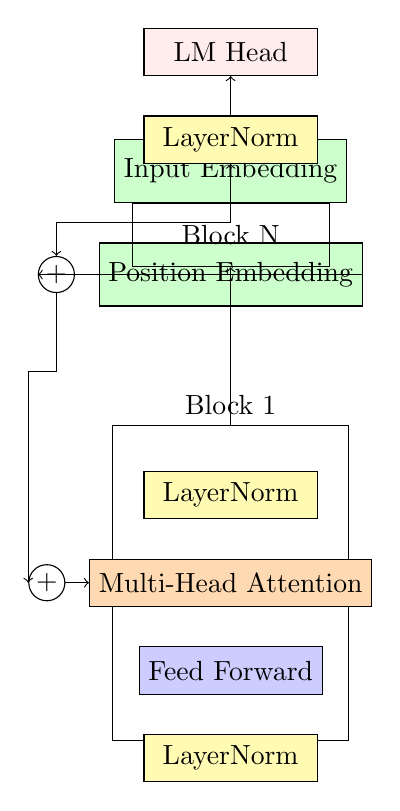
\begin{tikzpicture}[node distance=5mm]

% Input embedding
\node[block, fill=green!20] (input) {Input Embedding};
\node[block, fill=green!20, below=of input] (pos) {Position Embedding};
\node[add, left=3mm of pos] (add1) {+};
\draw[->] (input.south) -- ++(0,-0.25) -| (add1.north);
\draw[->] (pos.east) -- (add1.west);

% Block 1 (Transformer encoder/decoder style)
\node[draw, rectangle, minimum width=3cm, minimum height=4cm, below=1.5cm of pos, label=above:Block 1] (block1) {};

\node[smallblock, fill=orange!30] (attn) at (block1.center) {Multi-Head Attention};
\node[smallblock, fill=yellow!30, above=of attn] (ln1) {LayerNorm};
\node[smallblock, fill=blue!20, below=of attn] (ff) {Feed Forward};
\node[smallblock, fill=yellow!30, below=of ff] (ln2) {LayerNorm};

% Residual connections inside block
\node[add, left=3mm of attn] (add2) {+};
\draw[->] (add1.south) -- ++(0,-1) -| (add2.west);
\draw[->] (add2.east) -- (attn.west);

% Block N
\node[block, above=2cm of block1.north] (blockn) {Block N};
\node[smallblock, fill=yellow!30, above=of blockn] (ln3) {LayerNorm};
\node[smallblock, fill=pink!30, above=of ln3] (lm) {LM Head};

% Arrows through top
\draw[->] (block1.north) -- (blockn.south);
\draw[->] (blockn.north) -- (ln3.south);
\draw[->] (ln3.north) -- (lm.south);

\end{tikzpicture}
\end{document}
